\documentclass{article}
\usepackage[preprint, nonatbib]{neurips_2026}
\usepackage{microtype}
\usepackage{url}
\usepackage{pdfpages}
\usepackage{fancyhdr}
\usepackage{geometry}

\pagestyle{plain}

\title{Every Token of \texttt{cl100k\_base} in \texttt{tiktoken}}
\author{
  Z. Cheng \\
  \texttt{marc.cheng@alumni.utoronto.ca}
}

\begin{document}
\maketitle
\thispagestyle{plain}

\begin{abstract}
\begin{center}
We enumerate every token in \texttt{cl100k\_base} using \texttt{tiktoken}.
\end{center}
\end{abstract}

\section{Introduction}
\texttt{cl100k\_base} is the tokenizer underlying GPT-4 \cite{openai2023gpt4}
and related models.
It has 100,277 tokens \cite{tiktoken}.

\section{Background}
Byte Pair Encoding \cite{sennrich2016neural} produces a vocabulary
by iteratively merging the most frequent byte pair in a training corpus
until a target vocabulary size is reached.

\section{Methodology}
Each integer $i \in [0,\ 100{,}276]$ was mapped to its corresponding byte sequence, then decoded as UTF-8 where possible. Time complexity is $O(n)$. Space complexity is $O(n)$.

Tokens that are not valid UTF-8 in isolation are displayed as raw byte
literals; special tokens and unassigned IDs are annotated accordingly.

\section{Findings}
The training corpus is mostly English.

\section{Conclusion}
The vocabulary is finite.

\section*{Acknowledgments}
The author thanks the vocabulary for being finite.

\begin{thebibliography}{9}
\bibitem{openai2023gpt4}
OpenAI.
\newblock {GPT-4} Technical Report, 2023.
\newblock \url{https://arxiv.org/abs/2303.08774}

\bibitem{tiktoken}
OpenAI.
\newblock tiktoken, 2023.
\newblock \url{https://github.com/openai/tiktoken}

\bibitem{sennrich2016neural}
Rico Sennrich, Barry Haddow, and Alexandra Birch.
\newblock Neural Machine Translation of Rare Words with Subword Units.
\newblock In \textit{Proceedings of ACL}, 2016.
\end{thebibliography}

{
  \newgeometry{bottom=1.8cm}
  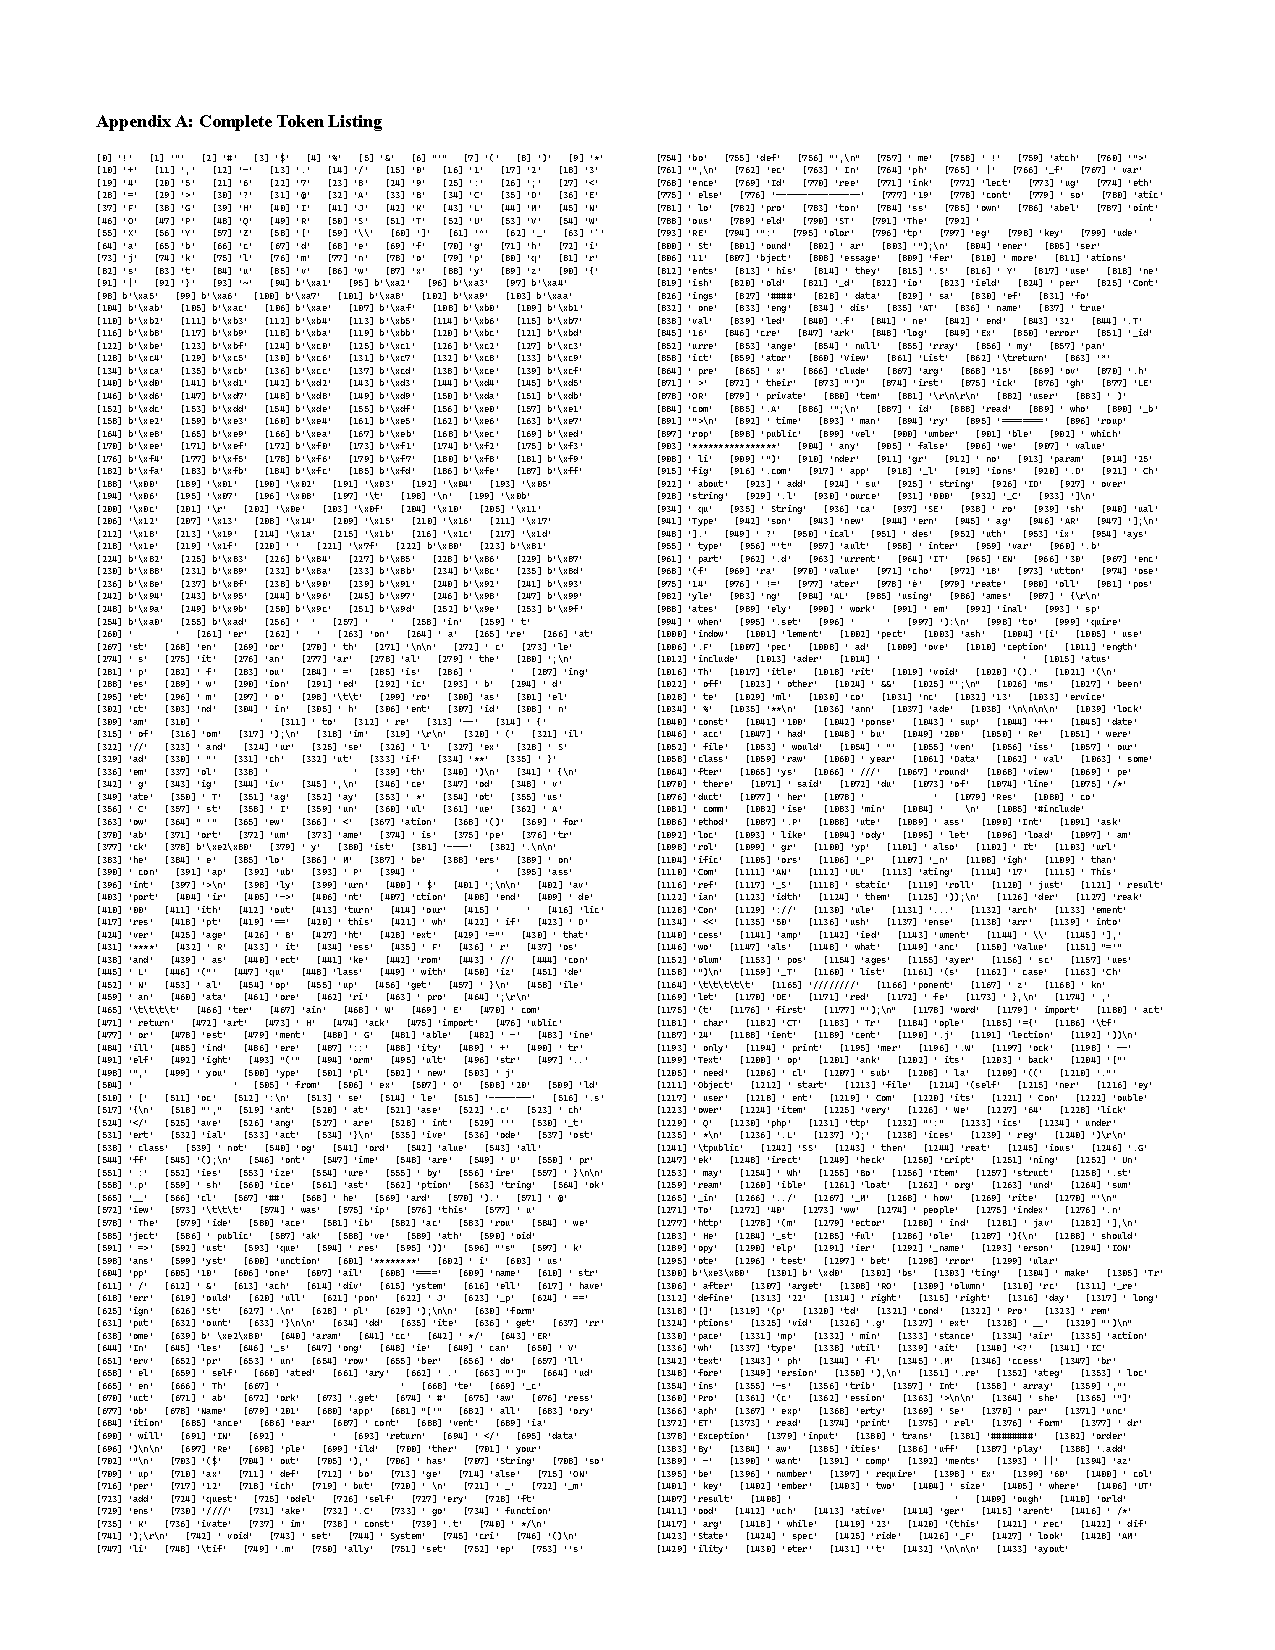
\includepdf[pages=-, pagecommand={\thispagestyle{plain}}]{appendix.pdf}
  \restoregeometry
}

\end{document}